\documentclass[border=10pt]{standalone}
\usepackage{tikz}
\begin{document}
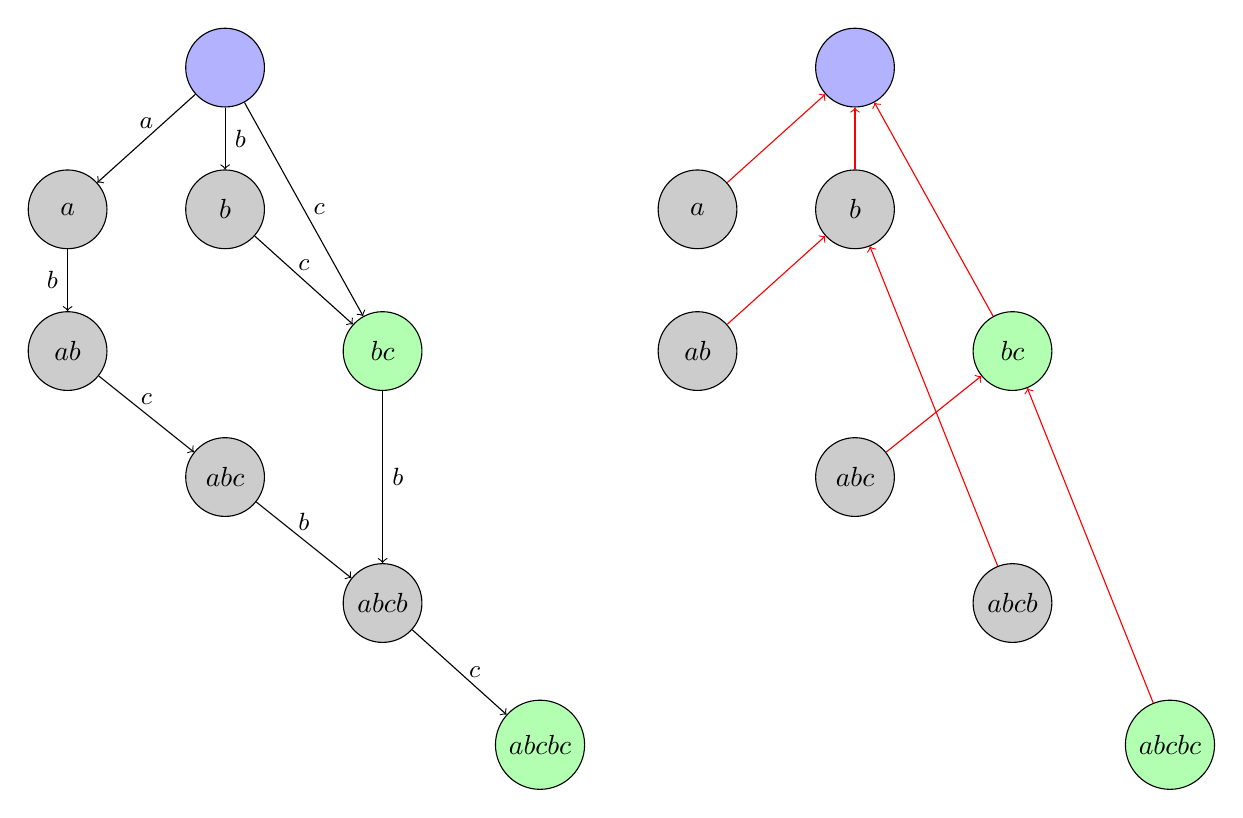
\begin{tikzpicture}[->,sibling distance=10em,
    every node/.style = {shape=circle, rounded corners,
    draw, align=center,minimum size=1.0cm, fill=black!20},
    cgreen/.style={fill=green!30},
    cblue/.style={fill=blue!30}]]
    \node[cblue] (1) at (0, 0) {$$};
    \node (2) at (-2, -1.8) {$a$};
    \node (3) at (0, -1.8) {$b$};
    \node[cgreen] (4) at (2, -3.6) {$bc$};
    \node (5) at (-2, -3.6) {$ab$};
    \node (6) at (0, -5.2) {$abc$};
    \node (7) at (2, -6.8) {$abcb$};
    \node[cgreen] (8) at (4, -8.6) {$abcbc$};
    \path[every node/.style={font=\sffamily\small}]
        (1) edge node[above] {$a$} (2)
        (1) edge node[right] {$b$} (3)
        (1) edge node[right] {$c$} (4)
        (2) edge node[left] {$b$} (5)
        (5) edge node[above] {$c$} (6)
        (6) edge node[above] {$b$} (7)
        (4) edge node[right] {$b$} (7)
        (7) edge node[right] {$c$} (8)
        (3) edge node[above] {$c$} (4);
    \node[cblue] (l1) at (8, 0) {$$};
    \node (l2) at (6, -1.8) {$a$};
    \node (l3) at (8, -1.8) {$b$};
    \node[cgreen] (l4) at (10, -3.6) {$bc$};
    \node (l5) at (6, -3.6) {$ab$};
    \node (l6) at (8, -5.2) {$abc$};
    \node (l7) at (10, -6.8) {$abcb$};
    \node[cgreen] (l8) at (12, -8.6) {$abcbc$};
    \path[every node/.style={font=\sffamily\small}]
        (l2) edge[red] node[above] {} (l1)
        (l3) edge[red] node[right] {} (l1)
        (l4) edge[red] node[right] {} (l1)
        (l5) edge[red] node[left] {} (l3)
        (l6) edge[red] node[above] {} (l4)
        (l7) edge[red] node[right] {} (l3)
        (l8) edge[red] node[above] {} (l4);
\end{tikzpicture}
\end{document}
